\documentclass[a4paper, 12pt]{book}

\usepackage[utf8x]{inputenc}   % omogoča uporabo slovenskih črk kodiranih v formatu UTF-8
\usepackage[slovene,english]{babel}    % naloži, med drugim, slovenske delilne vzorce
\usepackage[pdftex]{graphicx}  % omogoča vlaganje slik različnih formatov
\usepackage{fancyhdr}          % poskrbi, na primer, za glave strani
\usepackage{amssymb}           % dodatni simboli
\usepackage{amsmath}           % eqref, npr.
%\usepackage{hyperxmp}
\usepackage[hyphens]{url}  % dodal Solina
\usepackage{comment}       % dodal Solina

\usepackage[pdftex, colorlinks=true,
						citecolor=black, filecolor=black, 
						linkcolor=black, urlcolor=black,
						pagebackref=false, 
						pdfproducer={LaTeX}, pdfcreator={LaTeX}, hidelinks]{hyperref}

\usepackage{color}      
\usepackage{soul} 
\usepackage[numbers]{natbib}

%%%%%%%%%%%%%%%%%%%%%%%%%%%%%%%%%%%%%%%%
%	DIPLOMA INFO
%%%%%%%%%%%%%%%%%%%%%%%%%%%%%%%%%%%%%%%%
% \newcommand{\fixspacing}{\vspace{0pt plus 1filll}\mbox{}}

\newcommand{\ttitle}{Različni pristopi umetne inteligence v video igrah}
\newcommand{\ttitleEn}{Different Artificial intelligence approaches in video games}
\newcommand{\tsubject}{\ttitle}
\newcommand{\tsubjectEn}{\ttitleEn}
\newcommand{\tauthor}{Jovan Prodanov}
\newcommand{\tkeywords}{računalniška igra, umetna inteligenca, računalnik, pristopi}
\newcommand{\tkeywordsEn}{computer game, artificial intelligence, computer, approaches}

\usepackage{hyperref}
%%%%%%%%%%%%%%%%%%%%%%%%%%%%%%%%%%%%%%%%
%	HYPERREF SETUP
%%%%%%%%%%%%%%%%%%%%%%%%%%%%%%%%%%%%%%%%
\hypersetup{pdftitle={\ttitle}}
\hypersetup{pdfsubject=\ttitleEn}
\hypersetup{pdfauthor={\tauthor, jp6957@student.uni-lj.si}}
\hypersetup{pdfkeywords=\tkeywordsEn}

%%%%%%%%%%%%%%%%%%%%%%%%%%%%%%%%%%%%%%%%
% PAGE SETUP
%%%%%%%%%%%%%%%%%%%%%%%%%%%%%%%%%%%%%%%% 
\addtolength{\marginparwidth}{-20pt} % robovi za tisk
\addtolength{\oddsidemargin}{40pt}
\addtolength{\evensidemargin}{-40pt}

\renewcommand{\baselinestretch}{1.3} % ustrezen razmik med vrsticami
\setlength{\headheight}{15pt}        % potreben prostor na vrhu
\renewcommand{\chaptermark}[1]
{\markboth{\MakeUppercase{\thechapter.\ #1}}{}} \renewcommand{\sectionmark}[1]
{\markright{\MakeUppercase{\thesection.\ #1}}} \renewcommand{\headrulewidth}{0.5pt} \renewcommand{\footrulewidth}{0pt}
\fancyhf{}
\fancyhead[LE,RO]{\sl \thepage} 
%\fancyhead[LO]{\sl \rightmark} \fancyhead[RE]{\sl \leftmark}
\fancyhead[RE]{\sc \tauthor}              % dodal Solina
\fancyhead[LO]{\sc Bachelor's thesis}     % dodal Solina

\newcommand{\BibTeX}{{\sc Bib}\TeX}

%%%%%%%%%%%%%%%%%%%%%%%%%%%%%%%%%%%%%%%%
% TITLES
%%%%%%%%%%%%%%%%%%%%%%%%%%%%%%%%%%%%%%%%  
\newcommand{\autfont}{\Large}
\newcommand{\titfont}{\LARGE\bf}
\newcommand{\clearemptydoublepage}{\newpage{\pagestyle{empty}\cleardoublepage}}
\setcounter{tocdepth}{1}	      % globina kazala

%%%%%%%%%%%%%%%%%%%%%%%%%%%%%%%%%%%%%%%%
% CONSTRUCTORS
%%%%%%%%%%%%%%%%%%%%%%%%%%%%%%%%%%%%%%%%  
% \newtheorem{izrek}{Izrek}[chapter]
% \newtheorem{trditev}{Trditev}[izrek]
% \newenvironment{dokaz}{\emph{Dokaz.}\ }{\hspace{\fill}{$\Box$}}

%%%%%%%%%%%%%%%%%%%%%%%%%%%%%%%%%%%%%%%%%%%%%%%%%%%%%%%%%%%%%%%%%%%%%%%%%%%%%%%
%% PDF-A
%%%%%%%%%%%%%%%%%%%%%%%%%%%%%%%%%%%%%%%%%%%%%%%%%%%%%%%%%%%%%%%%%%%%%%%%%%%%%%%

%%%%%%%%%%%%%%%%%%%%%%%%%%%%%%%%%%%%%%%% 
% define medatata
%%%%%%%%%%%%%%%%%%%%%%%%%%%%%%%%%%%%%%%% 
\def\Title{\ttitle}
\def\Author{\tauthor, ales.jaklic@fri.uni-lj.si}
\def\Subject{\ttitleEn}
\def\Keywords{\tkeywordsEn}

%%%%%%%%%%%%%%%%%%%%%%%%%%%%%%%%%%%%%%%% 
% \convertDate converts D:20080419103507+02'00' to 2008-04-19T10:35:07+02:00
%%%%%%%%%%%%%%%%%%%%%%%%%%%%%%%%%%%%%%%% 
\def\convertDate{%
    \getYear
}

{\catcode`\D=12
 \gdef\getYear D:#1#2#3#4{\edef\xYear{#1#2#3#4}\getMonth}
}
\def\getMonth#1#2{\edef\xMonth{#1#2}\getDay}
\def\getDay#1#2{\edef\xDay{#1#2}\getHour}
\def\getHour#1#2{\edef\xHour{#1#2}\getMin}
\def\getMin#1#2{\edef\xMin{#1#2}\getSec}
\def\getSec#1#2{\edef\xSec{#1#2}\getTZh}
\def\getTZh +#1#2{\edef\xTZh{#1#2}\getTZm}
\def\getTZm '#1#2'{%
    \edef\xTZm{#1#2}%
    \edef\convDate{\xYear-\xMonth-\xDay T\xHour:\xMin:\xSec+\xTZh:\xTZm}%
}

%\expandafter\convertDate\pdfcreationdate 

%%%%%%%%%%%%%%%%%%%%%%%%%%%%%%%%%%%%%%%%
% get pdftex version string
%%%%%%%%%%%%%%%%%%%%%%%%%%%%%%%%%%%%%%%% 
\newcount\countA
\countA=\pdftexversion
\advance \countA by -100
\def\pdftexVersionStr{pdfTeX-1.\the\countA.\pdftexrevision}


%%%%%%%%%%%%%%%%%%%%%%%%%%%%%%%%%%%%%%%%
% XMP data
%%%%%%%%%%%%%%%%%%%%%%%%%%%%%%%%%%%%%%%%  
\usepackage{xmpincl}
%\includexmp{pdfa-1b}

%%%%%%%%%%%%%%%%%%%%%%%%%%%%%%%%%%%%%%%%
% pdfInfo
%%%%%%%%%%%%%%%%%%%%%%%%%%%%%%%%%%%%%%%%  
\pdfinfo{%
    /Title    (\ttitle)
    /Author   (\tauthor, jp6957@student.uni-lj.si)
    /Subject  (\ttitleEn)
    /Keywords (\tkeywordsEn)
    /ModDate  (\pdfcreationdate)
    /Trapped  /False
}


%%%%%%%%%%%%%%%%%%%%%%%%%%%%%%%%%%%%%%%
% START
%%%%%%%%%%%%%%%%%%%%%%%%%%%%%%%%%%%%%%%
\begin{document}
\selectlanguage{english}
\frontmatter
\setcounter{page}{1} %
\renewcommand{\thepage}{}       % preprecimo težave s številkami strani v kazalu
\newcommand{\sn}[1]{"`#1"'}                    % dodal Solina (slovenski narekovaji)

%%%%%%%%%%%%%%%%%%%%%%%%%%%%%%%%%%%%%%%%
% INTRO
%%%%%%%%%%%%%%%%%%%%%%%%%%%%%%%%%%%%%%%%
 \thispagestyle{empty}%
   \begin{center}
    {\large\sc Univerza v Ljubljani\\%
      Fakulteta za računalništvo in informatiko}%
    \vskip 10em%
    {\autfont \tauthor\par}%
    {\titfont \ttitle \par}%
    {\vskip 2em \textsc{DIPLOMSKO DELO\\[2mm]
    VISOKOŠOLSKI STROKOVNI ŠTUDIJSKI PROGRAM PRVE STOPNJE RAČUNALNIŠTVO IN INFORMATIKA}\par}%
    \vfill\null%
    {\large \textsc{Mentor}: doc.\ dr.  Aleš Jaklič\par}%
    {\vskip 2em \large Ljubljana, 2022 \par}%
\end{center}

\clearemptydoublepage

%%%%%%%%%%%%%%%%%%%%%%%%%%%%%%%%%%%%%%%%
% INTRO ENGLISH
%%%%%%%%%%%%%%%%%%%%%%%%%%%%%%%%%%%%%%%%
 \thispagestyle{empty}%
   \begin{center}
    {\large\sc University of Ljubljana\\%
      Faculty of Computer and Information Science}%
    \vskip 10em%
    {\autfont \tauthor\par}%
    {\titfont \ttitleEn \par}%
    {\vskip 2em \textsc{Bachelor's Thesis\\[2mm]
    UNIVERSITY STUDY PROGRAMME UNDERGRADUATE PROGRAMMES COMPUTER AND INFORMATION SCIENCE}\par}%
    % Not sure if correct "University"
    \vfill\null%
    {\large \textsc{Mentor}: doc.\ dr.  Aleš Jaklič\par}%
    {\vskip 2em \large Ljubljana, 2022 \par}%
\end{center}


%%%%%%%%%%%%%%%%%%%%%%%%%%%%%%%%%%%%%%%%
% copyright page
%%%%%%%%%%%%%%%%%%%%%%%%%%%%%%%%%%%%%%%%
\thispagestyle{empty}
\vspace*{8cm}

\noindent
{\sc Copyright}. 
Rezultati diplomske naloge so intelektualna lastnina avtorja in matične fakultete Univerze v Ljubljani.
Za objavo in koriščenje rezultatov diplomske naloge je potrebno pisno privoljenje avtorja, fakultete ter mentorja.

\begin{center}
\mbox{}\vfill
\emph{Besedilo je oblikovano z urejevalnikom besedil \LaTeX.}
\end{center}
%%%%%%%%%%%%%%%%%%%%%%%%%%%%%%%%%%%%%%%%

\clearemptydoublepage

%%%%%%%%%%%%%%%%%%%%%%%%%%%%%%%%%%%%%%%%
% stran 3 med uvodnimi listi
\thispagestyle{empty}
\
\vfill

\bigskip
\noindent\textbf{Kandidat:} \tauthor\\
\noindent\textbf{Naslov:} \ttitle\\
\noindent\textbf{Vrsta naloge:} Diplomska naloga na visokošolskem programu prve stopnje Računalništvo in informatika \\
\noindent\textbf{Mentor:} doc. dr. Aleš Jaklič\\

\bigskip
\noindent\textbf{Opis:}\\
Raziskovanje različnih načinov uporabe umetne inteligence v računalniški igri. Od osnovnih stanj do algoritmov strojnega učenja. Cilj je poskušati primerjati rezultate različnih metod in ugotoviti najboljše.\\
Besedilo teme diplomskega dela študent prepiše iz študijskega informacijskega sistema, kamor ga je vnesel mentor. 
V nekaj stavkih bo opisal, kaj pričakuje od kandidatovega diplomskega dela. 
Kaj so cilji, kakšne metode naj uporabi, morda bo zapisal tudi ključno literaturo.

\bigskip
\noindent\textbf{Title:} \ttitleEn

\bigskip
\noindent\textbf{Description:}\\
Researching different ways of how Artificial intelligence is used in a computer game. From basic state machines to machine learning algorithms. The goal is trying to compare results of different methods and figure out the best ones.


\vfill

\vspace{2cm}

% prazna stran
\clearemptydoublepage

% zahvala
\thispagestyle{empty}\mbox{}\vfill\null\it%
\noindent
Zelo sem hvaležen vsem, ki so mi pomagali priti tja, kjer sem.
\rm\normalfont

% prazna stran
\clearemptydoublepage

%%%%%%%%%%%%%%%%%%%%%%%%%%%%%%%%%%%%%%%%
% posvetilo, če sama zahvala ne zadošča :-)
%%%%%%%%%%%%%%%%%%%%%%%%%%%%%%%%%%%%%%%%

\thispagestyle{empty}\mbox{}{\vskip0.20\textheight}\mbox{}\hfill\begin{minipage}{0.55\textwidth}%
Za svoja draga družina.
\normalfont\end{minipage}

% prazna stran
\clearemptydoublepage


%%%%%%%%%%%%%%%%%%%%%%%%%%%%%%%%%%%%%%%%
% kazalo
\pagestyle{empty}
\def\thepage{}% preprecimo tezave s stevilkami strani v kazalu
\tableofcontents{}


% prazna stran
\clearemptydoublepage


%%%%%%%%%%%%%%%%%%%%%%%%%%%%%%%%%%%%%%%%
% List of abbriviations
%%%%%%%%%%%%%%%%%%%%%%%%%%%%%%%%%%%%%%%%

% \chapter*{Seznam uporabljenih kratic}  % spremenil Solina, da predolge vrstice ne gredo preko desnega roba
\chapter*{List of abbreviations used}  % spremenil Solina, da predolge vrstice ne gredo preko desnega roba

\noindent\begin{tabular}{p{0.21\textwidth}|p{.4\textwidth}|p{.4\textwidth}}    % po potrebi razširi prvo kolono tabele na račun drugih dveh!
    % {\bf kratica} & {\bf angleško} & {\bf slovensko} \\ \hline
  {\bf Abbreviation} & {\bf English} & {\bf Slovenian} \\ \hline
  % after \\: \hline or \cline{col1-col2} \cline{col3-col4} ...
  {\bf ML}      & machine learning                  & strojno učenje \\
  {\bf FMS}     & finite state machine              & končni stroj \\
  {\bf NN}      & neural network                    & nevronska mreža \\
  {\bf CNN}     & convolutional neural network      & konvolucijska nevronska mreža \\
  {\bf NPC}     & non-player character              & neigralski lik \\
  {\bf CA}      & classification accuracy           & klasifikacijska točnost \\
  {\bf NPC }    & non-player character              & neigralski lik \\
  \dots         & \dots                             & \dots \\
\end{tabular}

% prazna stran
\clearemptydoublepage

%%%%%%%%%%%%%%%%%%%%%%%%%%%%%%%%%%%%%%%%
% povzetek
%%%%%%%%%%%%%%%%%%%%%%%%%%%%%%%%%%%%%%%%

\addcontentsline{toc}{chapter}{Povzetek}
\chapter*{Povzetek}

\noindent\textbf{Naslov:} \ttitle
\bigskip

\noindent\textbf{Avtor:} \tauthor
\bigskip

%\noindent\textbf{Povzetek:} 
\noindent 
V diplomski nalogi bodo predstavljeni različni načini uporabe umetne inteligence v računalniških igrah s poudarkom na orodju, ki deep reinforcement learning.
Ta diplomska naloga bo obravnavala načine ravnanja z umetno inteligenco v video igrah, kot so: FMS, mehka logika, skriptiranje, zbiranje, drevesa odločanja, vedenjska drevesa, nevronske mreže, genetski algoritmi.
Raziskoval bom zgoraj omenjene načine, naredil primere in predstavil njihove rezultate.
\bigskip

\noindent\textbf{Ključne besede:} \tkeywords.
% prazna stran
\clearemptydoublepage


%%%%%%%%%%%%%%%%%%%%%%%%%%%%%%%%%%%%%%%%
% abstract
%%%%%%%%%%%%%%%%%%%%%%%%%%%%%%%%%%%%%%%%

\selectlanguage{english}
\addcontentsline{toc}{chapter}{Abstract}
\chapter*{Abstract}

\noindent\textbf{Title:} \ttitleEn
\bigskip

\noindent\textbf{Author:} \tauthor
\bigskip

%\noindent\textbf{Abstract:} 
\noindent 
The thesis will present different ways of using artificial intelligence in computer games with an emphasis on a tool that uses deep reinforcement learning.
This thesis will handle ways of handling AI in video games like: FMS, Fuzzy logic, Scripting, Flocking, Decision trees, Behavioural trees, Neural networks, Genetics Algorithm.
I will research the above aforementioned ways, even make examples and present their results.
\bigskip



\noindent\textbf{Keywords:} \tkeywordsEn.
\selectlanguage{english}
% prazna stran
\clearemptydoublepage


%%%%%%%%%%%%%%%%%%%%%%%%%%%%%%%%%%%%%%%%
% START
%%%%%%%%%%%%%%%%%%%%%%%%%%%%%%%%%%%%%%%%

\mainmatter
\setcounter{page}{1}
\pagestyle{fancy}


\chapter{Introduction}

The AI problem in video games has been present for a long time, but as time goes on we are getting introduced new ways of solving it. But, game developers are still sticking to the old ways of doing things. % ew this is so cringe

In this thesis we will dive deeper into of the AI in games and figure out what's in store for the future of AI in video games.

In chapter \ref{ch1} we are going to get to know the problem and see how it came to be.
Chapter \ref{ch2} will explain the present situation and I will present a different technology that can be used in chapter \ref{ch3} and conclude in chapter \ref{ch4}.


\chapter{Background}
\label{ch1}
The question of game AI was present even in the first of games developed. By definition, in video games, AI is used to generate responsive, adaptive or intelligent behaviors primarily in NPCs similar to human-like intelligence \cite{AIwiki}. The ways of approaching it is incredibly vast, in this thesis we will only scratch the surface, but focus on the most interesting ones.

\section{What is AI in games?}
First, I should start with the term "video game", in definition it is an electronic game that involves interaction with a user interface or input device such as a joystick, controller, keyboard, or motion sensing device to generate visual feedback \cite{VideoGameWiki}. Then, the visual feedback is channeled to a displaying device, which can be observed. 

So, now for quite some time, game developers are trying to invent techniques and methods for incorporating intelligence into these video games. But, this AI is a broad term, in video games, it can mean: animation control, steering, flocking, pathfinding, planning, procedural generation, tactical and strategic thinking, learning \cite{FuzzyAIGames}, to name a few. Often game AI can be mistaken for "true AI", which is to display human cognitive skills associated with human thinking, learning and problem-solving.

Game AI adds another piece of the puzzle of defining AI and that is the illusion of intelligence. We would never want in a game an unbeatable ever-learning opponent, we would like a fun and easy experience, which isn't obviously stupid. Game AI in video games exists only to be fun and entertaining, so looking from this point, this is why the game developers are sticking to things that are predictable and working and aren't experimenting a whole lot, because who would want unexpected things happening in a game.

\section{Illusion of intelligence}
Now that the secret is out, game developers were and are inventing tricks and techniques to make the player believe that games have real intelligence \cite{IllusionOfIntelligece}. And instead of making the goal true intelligence, its the appearance of intelligence.

\subsection{Why does it work?}
The true reason why this illusion works is that players want to believe that there are glimmers of real human-like intelligence in their virtual worlds \cite{IllusionOfIntelligece}. Also, with their high expectations the players are easily forgiving.

Another reason why it works is because of anthropomorphism, which is an attribution of human motivation, characteristics, or behavior to inanimate objects, animals, or natural phenomenon, and these can be related to a phenomenon in animation. There is a research that a preschool 91\% of the times picked a character that is not a human being 
 \cite{AnthropomorphicCharacters}.

As previously stated, expectations have a high influence. Because of the placebo effect, if players are expecting a highly intelligent game, their enjoyment will be higher. This is the same as if people think they are eating a more expensive food or a drink, they are more likely to enjoy it.

\subsection{Selling it}
The illusion of intelligence work when there is a certain level of quality to it, and that quality is helped by \cite{IllusionOfIntelligece}:
\begin{itemize}
    \item The AI should have \textbf{animation and dialog}. These things help it to interact with the world and player, as well as making it more alive and present.
    \item Although animations help to achieve game AI, it should be done with quality. They should the smooth and human-like, instead of looking like a \textbf{robot}.
    \item \textbf{Have a reason to exist}, AI characters shouldn't always wait for the player to approach, they should have their own purpose. As well as their own motives, because the game world would be their home and reality and they should have their own states in it.
    \item The culmination of building a successful AI character would be for it to have its own \textbf{personality}. How the game developer leverages this powerful tool can complete change the feel of the game.
\end{itemize}


\section{Deterministic vs Non-deterministic}
It is in close connection to game AI that there exists two type of games. In a deterministic game, the course of the game depends only on the players’ decisions, but in a non-deterministic game, there’s some factor of randomness involved \cite{DeepLearningGO}.

For example, chess is a deterministic game, the outcome of the game is entirely based on the players' decisions. But, football is non-deterministic, the players can't reliably kick the ball exactly the same every time. In that sense, luck or randomness often makes the game more exciting, however too much randomness removes all influence of the player in game, which is rarely fun.


\chapter{Current AI in games}
\label{ch2}

So, advanced techniques for game AI have been spotted more often, for examples, there have been usages of Bayesian networks and neural networks for real-time strategy games, as well as evolutionary algorithms \cite{FuzzyAIGames}. But, in those cases the game seems to orbit around that as the main focus of the game itself. In other words, advanced techniques for game AI currently need a game to be build around them. Then, there is the problem of evolutionary algorithms needing a high computational and memory power. Also, the last problem would be their non-determinism, that just brings more problems to the table and game developers are reluctant to ship a game that is not tested enough.

In this chapter, we will focus more on the current techniques that are widely used, which finely sell the illusion of intelligence. Technologies I will use if I need to present examples are Unity for the game editor and game engine \cite{UnitySoftware}.

\section{Finite State Machines}

You want to create a side-scrolling platformer, and now you grab a pen and paper and start designing the flowchart. You draw a box for everything the hero can be doing: standing, jumping, ducking and diving. When some kind of input is given, for an example when a button is pressed, you draw an arrow to from that box, label it with the button, and connect it to the box it changes to \cite{GameProgrammingPattersFMS}.

\begin{figure}[h]
\begin{center}
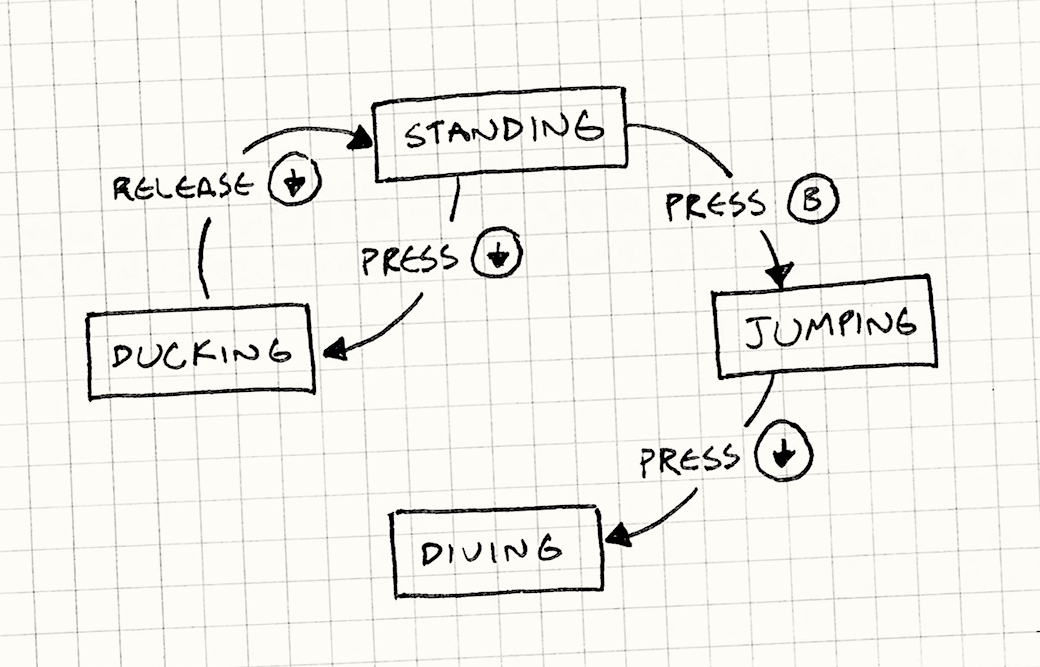
\includegraphics[width=0.6\textwidth]{Images/state_FSM.png}
\end{center}
\caption{Finite State Machine}
\label{pic1}
\end{figure}

Now that we successfully create a FSM, these came out of a computer science branch called automata theory, which includes the famous Turing machine. FSMs are the simplest of that bunch.

\begin{itemize}
    \item You have to have fixed set of states the machine can be in
    \item The machine can be in one state at a time
    \item Sequences of inputs or events are being sent to the machine
    \item Each state has a set of transitions, each associated  with an input/event and pointing to a state
\end{itemize}

So, now that I've introduced FSMs, there is a catch. State machines help you untangle hairy code by forcing a very constrained structure on it. All you have is a fixed set of states, a single current state, and some hardcoded transitions \cite{GameProgrammingPattersFMS}. However, when wanting to create a more complex game AI, you have to work around these problems, I'll close this chapter by presenting some. 

\subsection{Concurrent State Machines}

Let's now equip our hero with a gun. If we want to play by the constraints of an FSM, we have to double our states: standing, standing with a gun, jumping, jumping with a gun etc. Its redundant, however we can add another state into a single machine, what the hero is doing and what he's carrying.

\begin{verbatim}
class Hero  {
    private State _state;
    private State _equipment;

    private void HandleInput(Input input) {
        _state.HandleInput(input);
        _equipment.HandleInput(input);
    }
}
\end{verbatim}

\subsection{Hierarchical State Machines}

We wouldn't want to duplicate code in all of our states. We could define a state "on ground" that handles ducking and jumping, standing, walking, running would then inherit from that one and add it to its own behaviour.

Turns out this is a structure called hierarchical state machine, a state can have a superstate (making itself a substate). When an event comes in, if the substate doesn’t handle it, it rolls up the chain of superstates. In other words, it works just like overriding inherited methods \cite{GameProgrammingPattersFMS}.

If the current state is on top of the stack, under that is its superstate and so on. So, if you dish out a state-specific behaviour, it starts on top of the stack and walks down until one of the superstates handles it, but if none do, its ignored.

\subsection{Pushdown Automata}

This is an extension to FSM, that uses the concept of stacks. The problem is with basic FSMs is that you don't have history of the previous states. You know of what state you \emph{are} currenly in, but no memory of what state you \emph{were}.

So, if we had states standing and firing, if we were to transition in the firing state, we couldn't remember to go in our previous state, the standing state. For this problem, the pushdown automata structure is here to help.

In vanilla FSM, you have a singe pointer to the current state, pushdown automata has a stack of them. In a FSM, transitioning into the new state replaces the previous one. Pushdown automata let's you do that, but it gives you two other choices \cite{GameProgrammingPattersFMS}:

\begin{itemize}
    \item You can push a new state on the stack, the "current" state is always on top of the stack, so this transitions to the new state, but it leaves the previous state directly under the stack instead of discrading.
    \item You can pop the "current" state, in doing so, the state that is under it becomes the new "current" state.
\end{itemize}

\begin{figure}[h]
\begin{center}
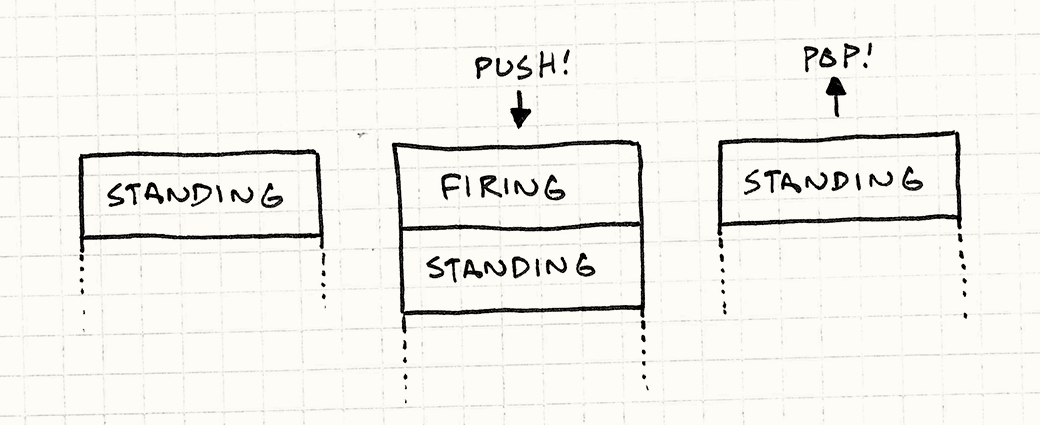
\includegraphics[width=0.6\textwidth]{Images/state_pushdown.png}
\end{center}
\caption{The Pushdown Automata}
\label{pic2}
\end{figure}

\section{Behavioural Trees}

Even with extensions to FSMs, they are pretty limited. If tha aim is complex game AI, the previous chapter only whet our appetite.

\section{Scripting}

\section{Fuzzy Logic}

\section{Flocking}

\section{Trees}

\section{Neural Networks?}

\section{Genetics Algorithm}

\chapter{ML-Agents}
\label{ch3}


\chapter{Conclusion}
\label{ch4}



\cleardoublepage
\addcontentsline{toc}{chapter}{Literature}
\bibliography{literature}
\bibliographystyle{plainnat}

\end{document}